\documentclass[main.tex]{article}
\usepackage{subfiles}
\usepackage{hyperref}
\usepackage{csquotes}
\usepackage{amsmath}
\usepackage{amsfonts}
\usepackage[]{geometry}
\usepackage{graphicx}
\usepackage{listings}
\usepackage{xcolor}
\usepackage{subcaption}

\graphicspath{{./figures/}}

\begin{document}
    \section[P6: Distributions from CDF]{Using inverse of CDF to generate different PDFs}
    All results are described in Figure \ref{fig:p6-cdfinv-pdf}.
    \subsection{Normal Distribution}
    The normal distribution's Probability Density Function (PDF) is given by
    \begin{equation}
        N(x; \mu, \sigma^2) = \frac{1}{\sqrt{2\pi \sigma^2}} \; \mathrm{exp} \left ( -\frac{(x-\mu)^2}{2\sigma^2} \right )
        \label{eq:normal-3}
    \end{equation}
    The Cumulative Density Function (CDF) for the above equation is given by
    \begin{equation}
        C_{N} (t; \mu, \sigma^2) = \frac{1}{2} \left ( 1 + \textup{erf} \left ( \frac{t-\mu}{\sqrt{2 \sigma^2}} \right ) \right )
    \end{equation}
    Where $\textup{erf}$ is the \emph{error function}, given by
    \begin{equation}
        \textup{erf}(t) = \frac{2}{\sqrt{\pi}} \int_{0}^{t} e^{-x^2} \mathrm{d}x
    \end{equation}
    The CDF equation $y = C_{N} (x; \mu, \sigma^2)$ can be inverted (get $x$ for given $y$) as follows
    \begin{equation}
        \begin{split}
            y & = \frac{1}{2} \left ( 1 + \textup{erf} \left ( \frac{x-\mu}{\sqrt{2 \sigma^2}} \right ) \right )
            \Rightarrow \textup{erf} \left ( \frac{x-\mu}{\sqrt{2 \sigma^2}} \right ) = 2y-1 \\
            & \Rightarrow \frac{x-\mu}{\sqrt{2 \sigma^2}} = \textup{erfinv} \left ( 2y-1 \right )
            \Rightarrow x = \mu + \sqrt{2\sigma^2} \, \textup{erfinv} \left ( 2y-1 \right )
        \end{split}
    \end{equation}
    Note that $\textup{erfinv}$ is the \emph{inverse of the error function}.
    \par Generating PDF through this is explored in Figure \ref{fig:p6-cdfinv-pdf-normal} with the corresponding code in \ref{app:code-p6-normal}.
    \subsection{Rayleigh Distribution}
    The Rayleigh distribution's Probability Density Function is given by
    \begin{equation}
        R(x; \sigma^2) = \frac{x}{\sigma^2} \, \textup{exp} \left ( \frac{-x^2}{2\sigma^2} \right ) \;\;\; x \ge 0
    \end{equation}
    The Cumulative Density Function for the above equation is given by
    \begin{equation}
        C_R (t; \sigma^2) = 1 - \textup{exp} \left ( \frac{-t^2}{2 \sigma^2} \right ) \;\;\; t \ge 0
    \end{equation}
    The CDF equation $y =  C_R (x; \sigma^2)$ can be inverted as follows
    \begin{equation}
        \begin{split}
            y & = 1 - \textup{exp} \left ( \frac{-x^2}{2 \sigma^2} \right ) 
            \Rightarrow (1-y) = \textup{exp} \left ( \frac{-x^2}{2 \sigma^2} \right ) \\
            & \Rightarrow \frac{x^2}{2 \sigma^2} = -\ln(1-y) \Rightarrow x = \sigma \sqrt{-2 \ln (1-y)} \\
            & \Rightarrow x = \sqrt{2 \sigma^2 \,\ln \left ( \frac{1}{1-y} \right )}
        \end{split}
    \end{equation}
    Generating PDF through this is explored in Figure \ref{fig:p6-cdfinv-pdf-rayleigh} with the corresponding code in \ref{app:code-p6-rayleigh}.
    \subsection{Exponential Distribution}
    The Exponential distribution's Probability Density Function is given by
    \begin{equation}
        E(x; \lambda) = \lambda e^{-\lambda x} \;\;\;\; x \ge 0
    \end{equation}
    The Cumulative Density Function for the above equation is given by
    \begin{equation}
        C_E(t; \lambda) = 1 - e^{-\lambda t}
    \end{equation}
    The CDF equation $y = C_E(x;\lambda)$ can be inverted as follows
    \begin{equation}
        \begin{split}
            y & = 1 - e^{-\lambda x} \Rightarrow e^{-\lambda x} = 1 - y 
            \Rightarrow x = \frac{-1}{\lambda} \ln (1-y) \\
            & \Rightarrow x = \frac{1}{\lambda} \ln \left ( \frac{1}{1-y} \right )
        \end{split}
    \end{equation}
    Generating PDF through this is explored in Figure \ref{fig:p6-cdfinv-pdf-exp} with the corresponding code in \ref{app:code-p6-exp}.
    \begin{figure}
        \begin{subfigure}{.45\textwidth}
            \centering
            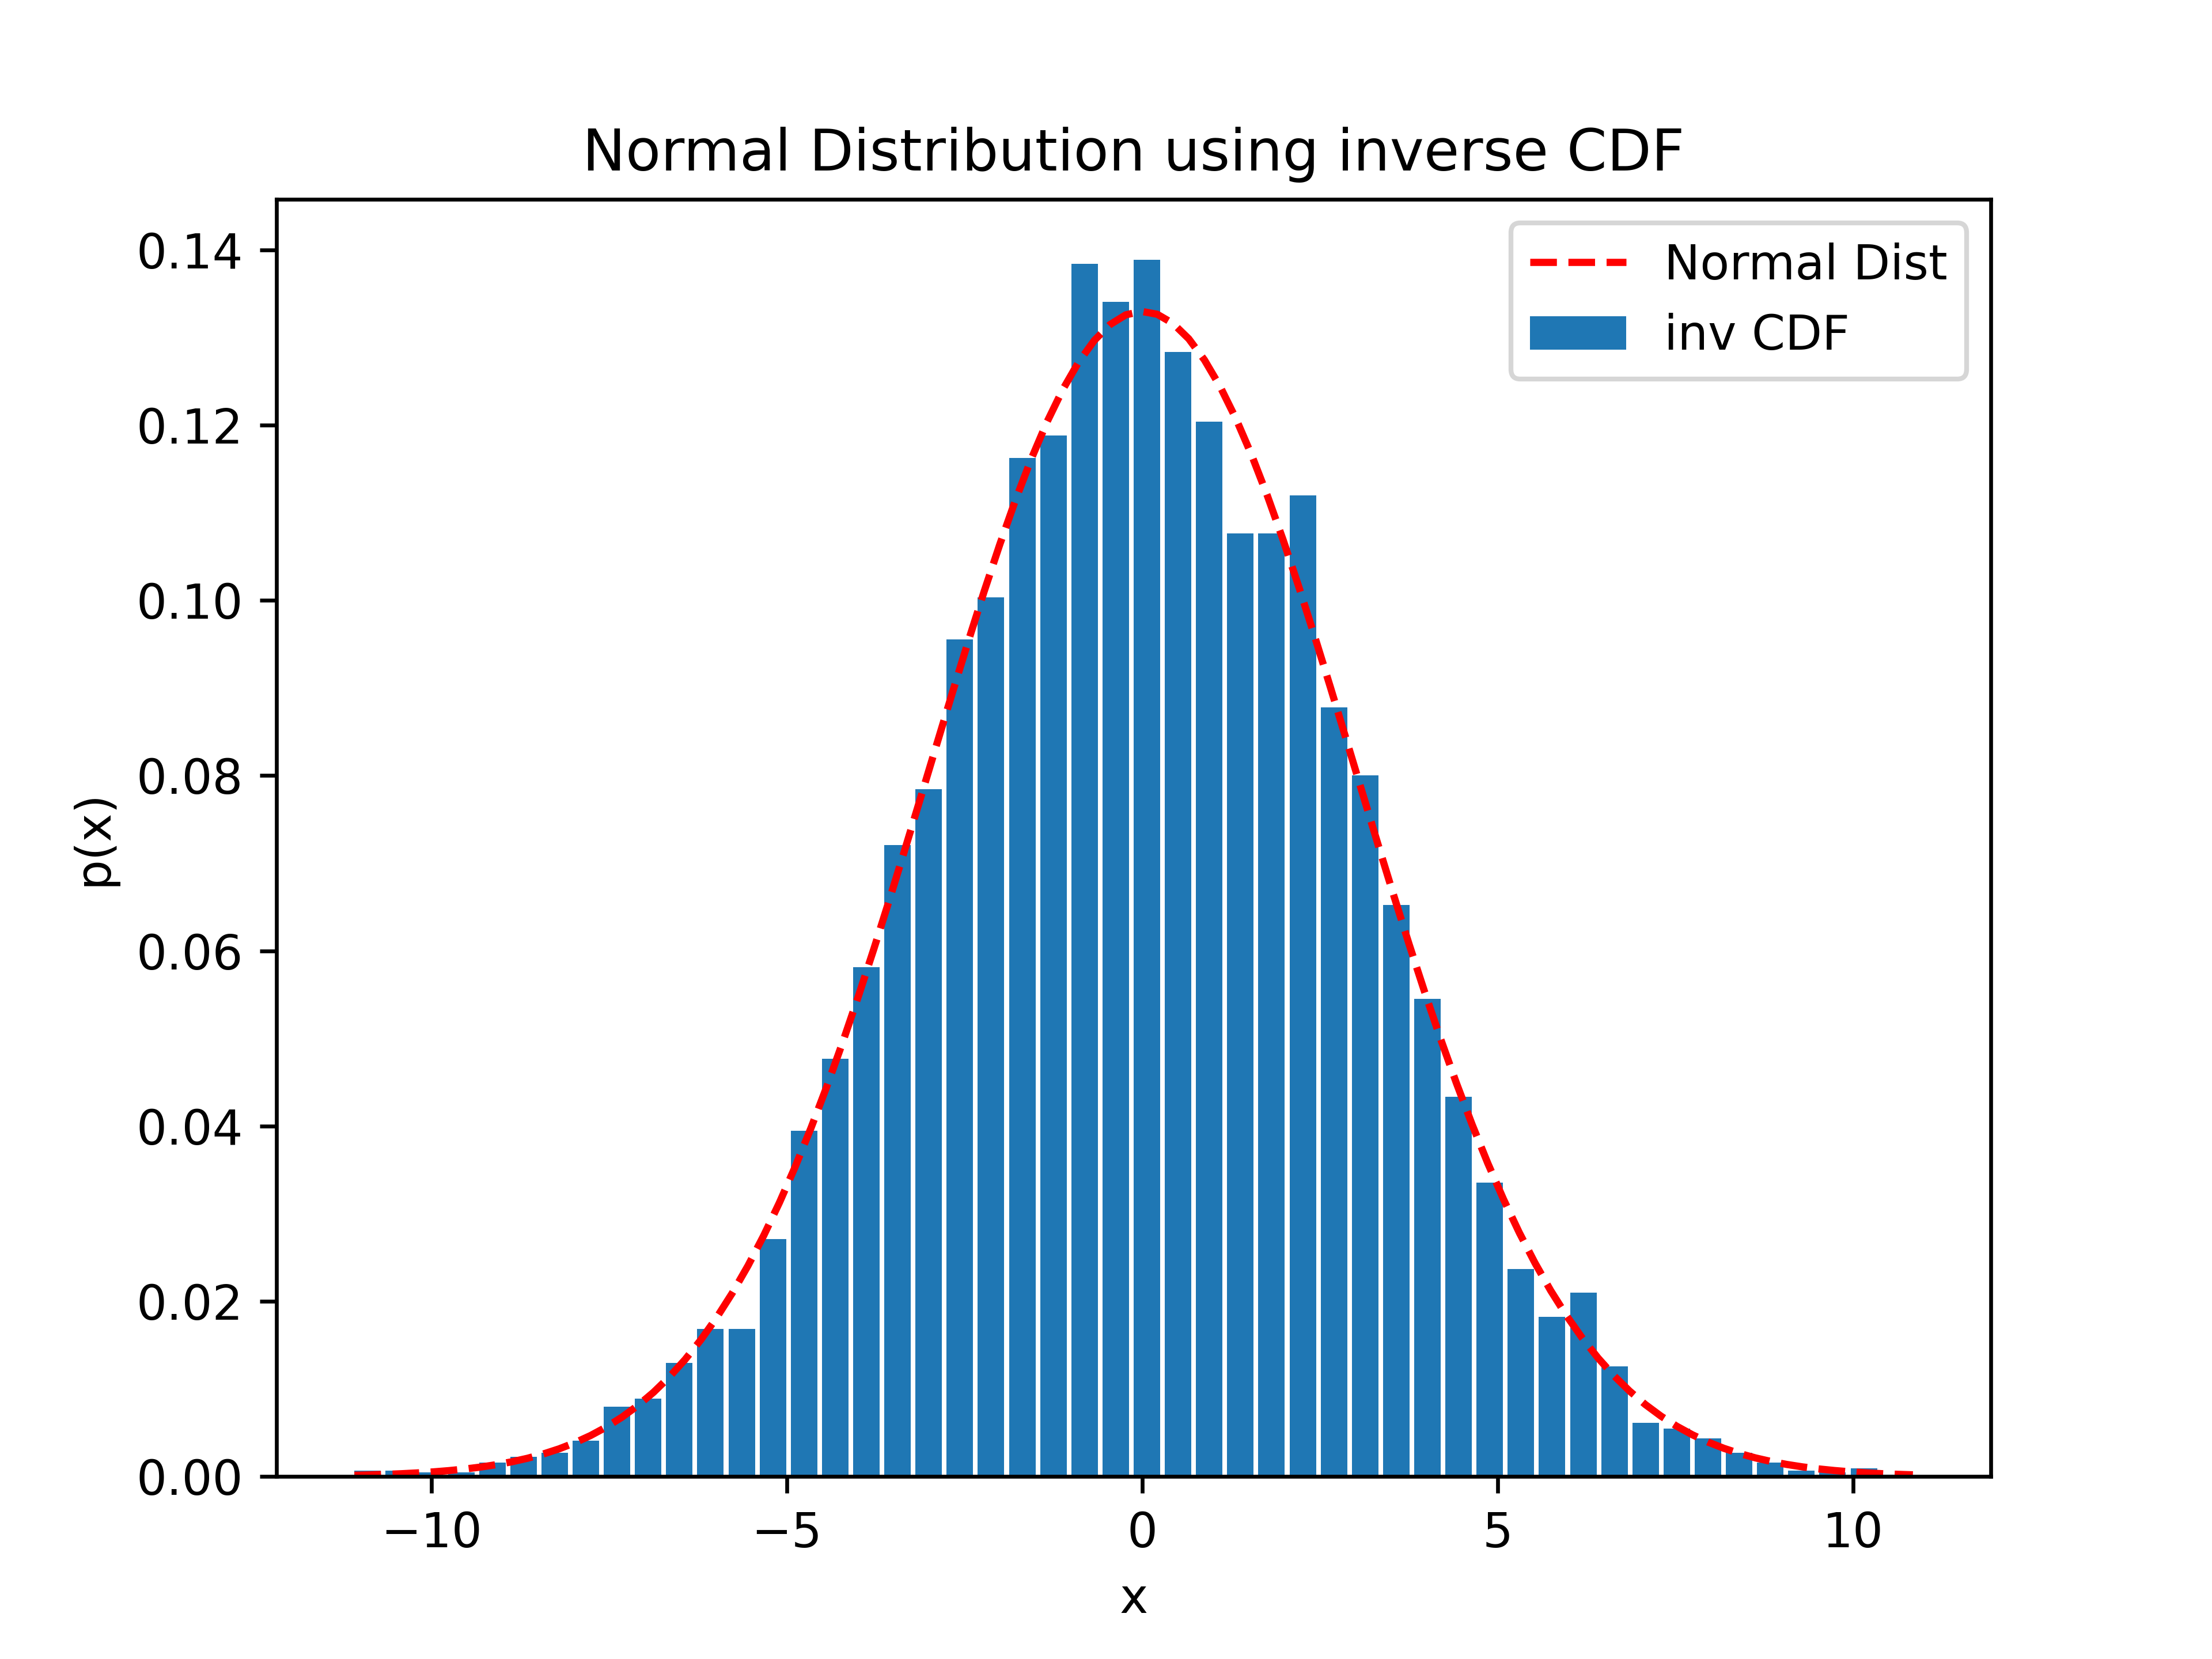
\includegraphics[width=.95\linewidth]{plot_p6_normal.png}
            \caption{$N(x; \mu = 0, \sigma^2 = 9)$}
            \label{fig:p6-cdfinv-pdf-normal}
        \end{subfigure}
        \begin{subfigure}{.45\linewidth}
            \centering
            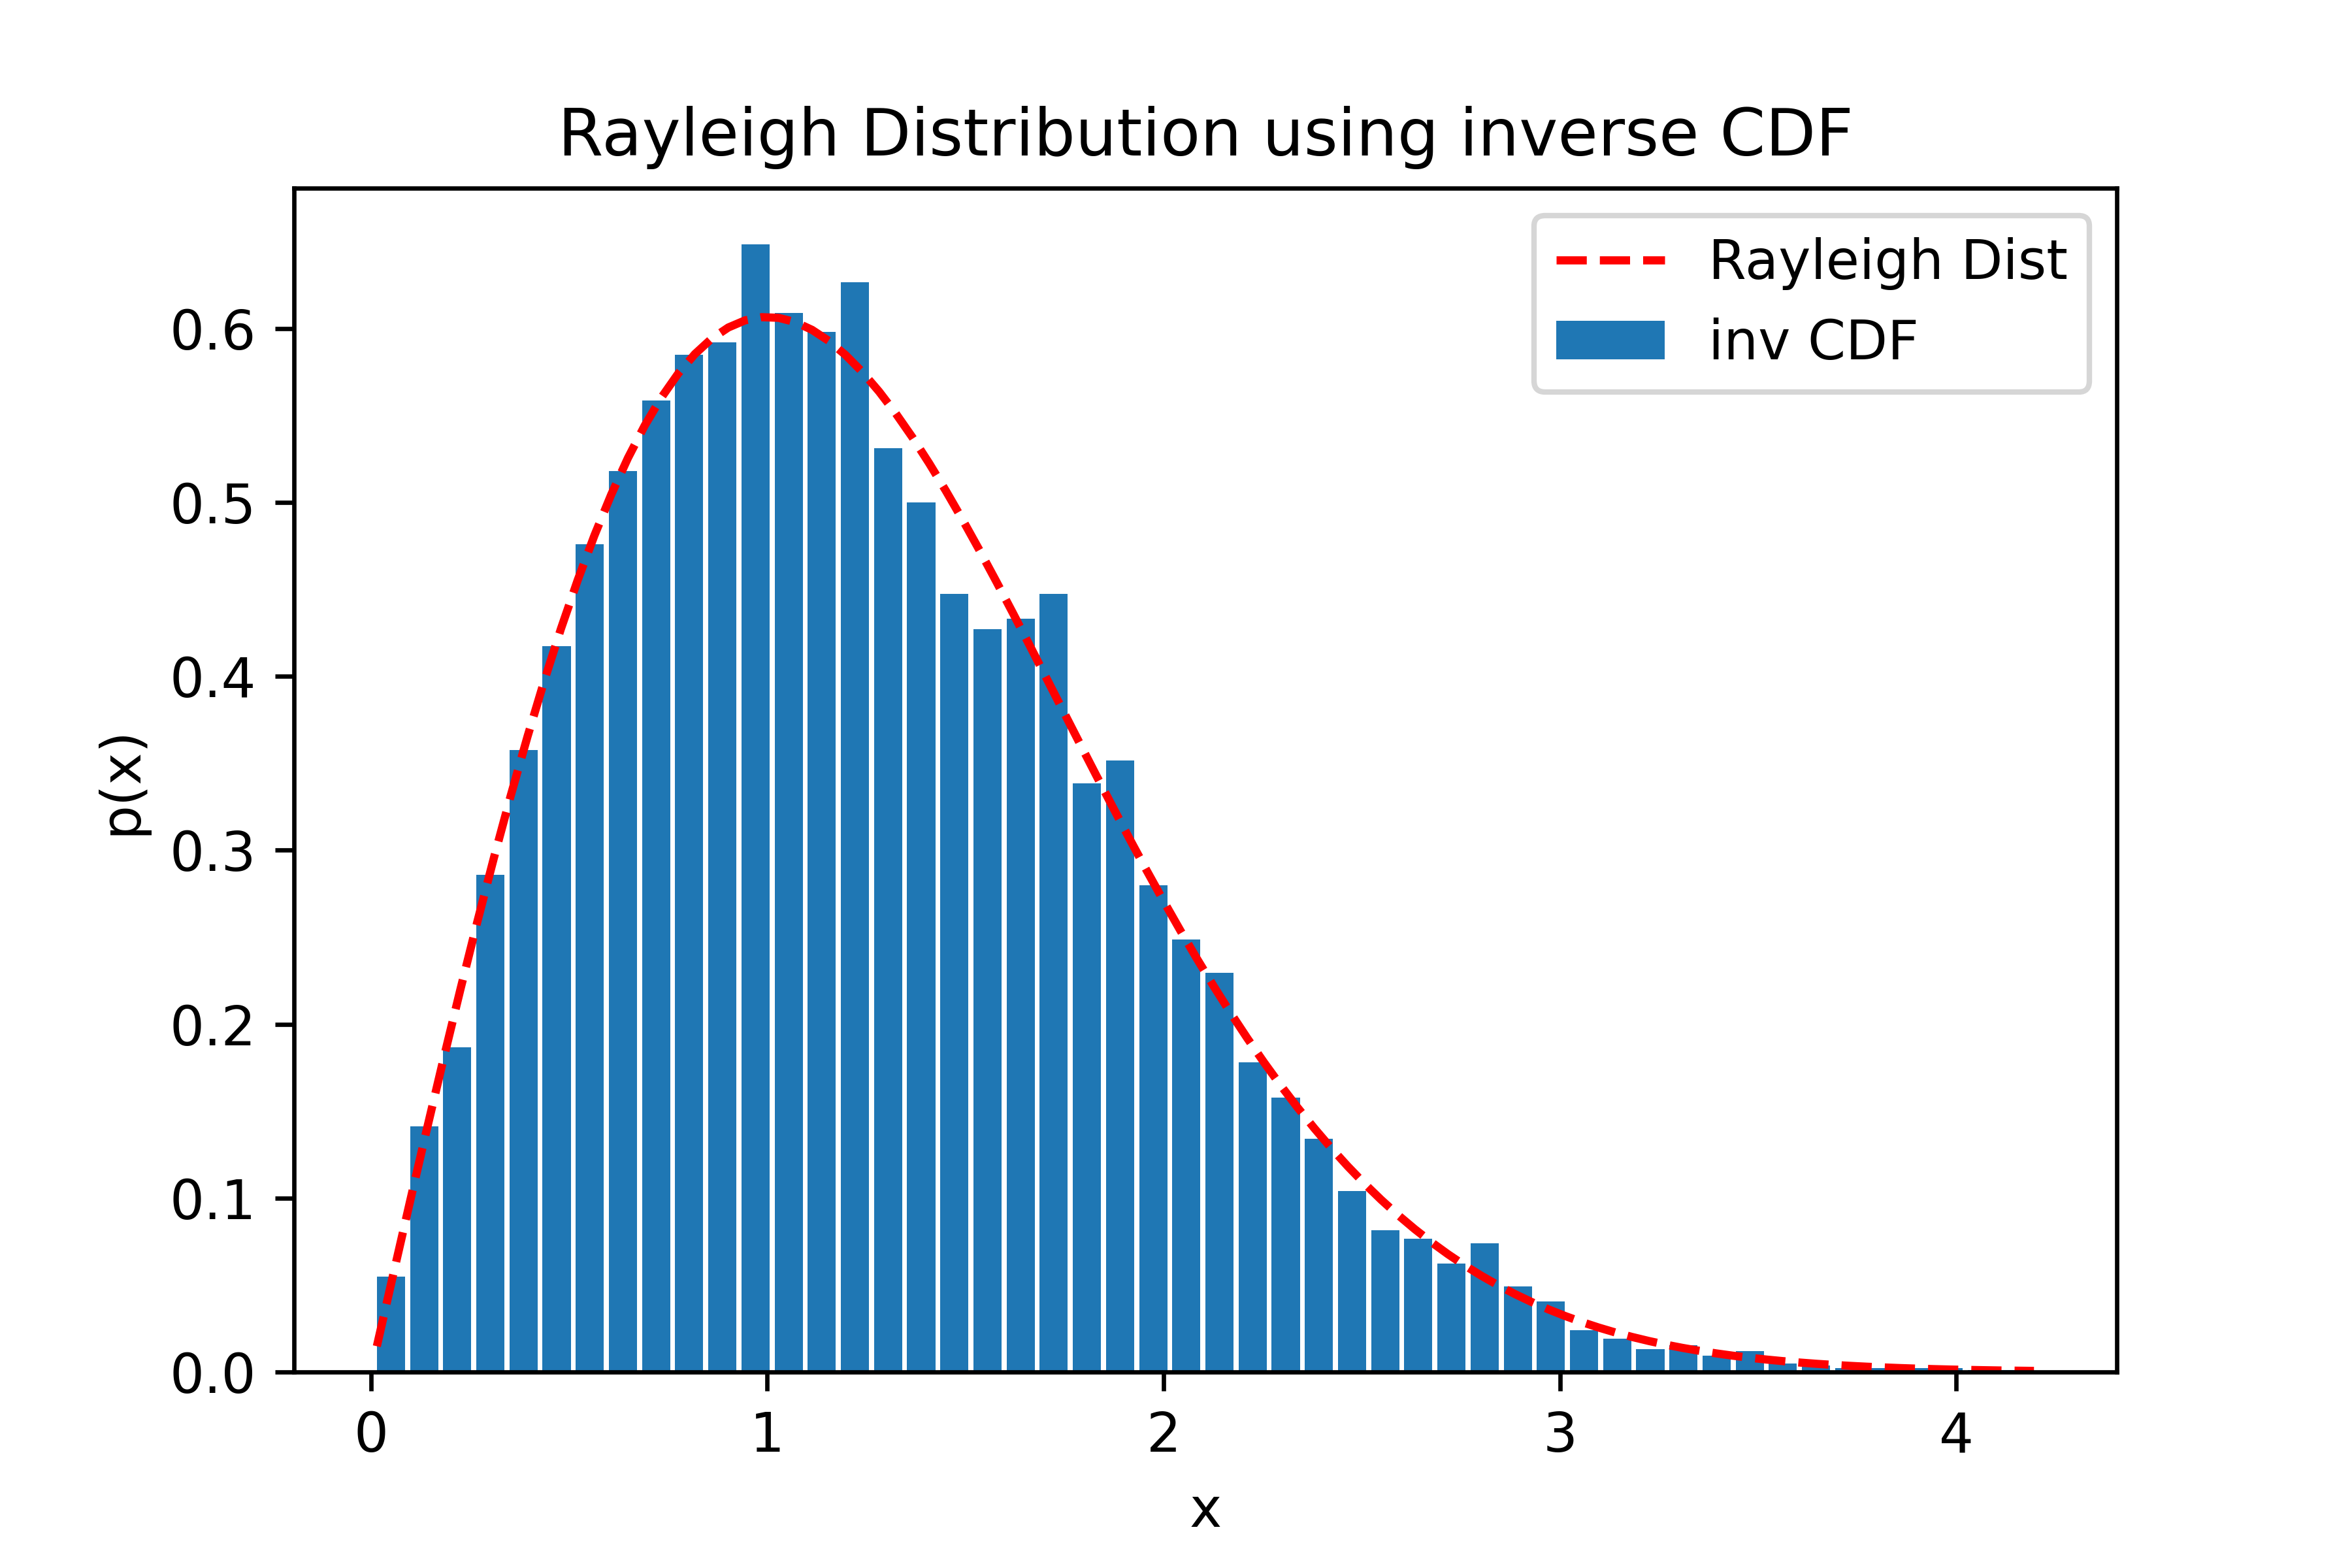
\includegraphics[width=.95\linewidth]{plot_p6_rayleigh.png}
            \caption{$R(x; \sigma^2 = 1)$}
            \label{fig:p6-cdfinv-pdf-rayleigh}
        \end{subfigure} \\
        \begin{subfigure}{.45\linewidth}
            \centering
            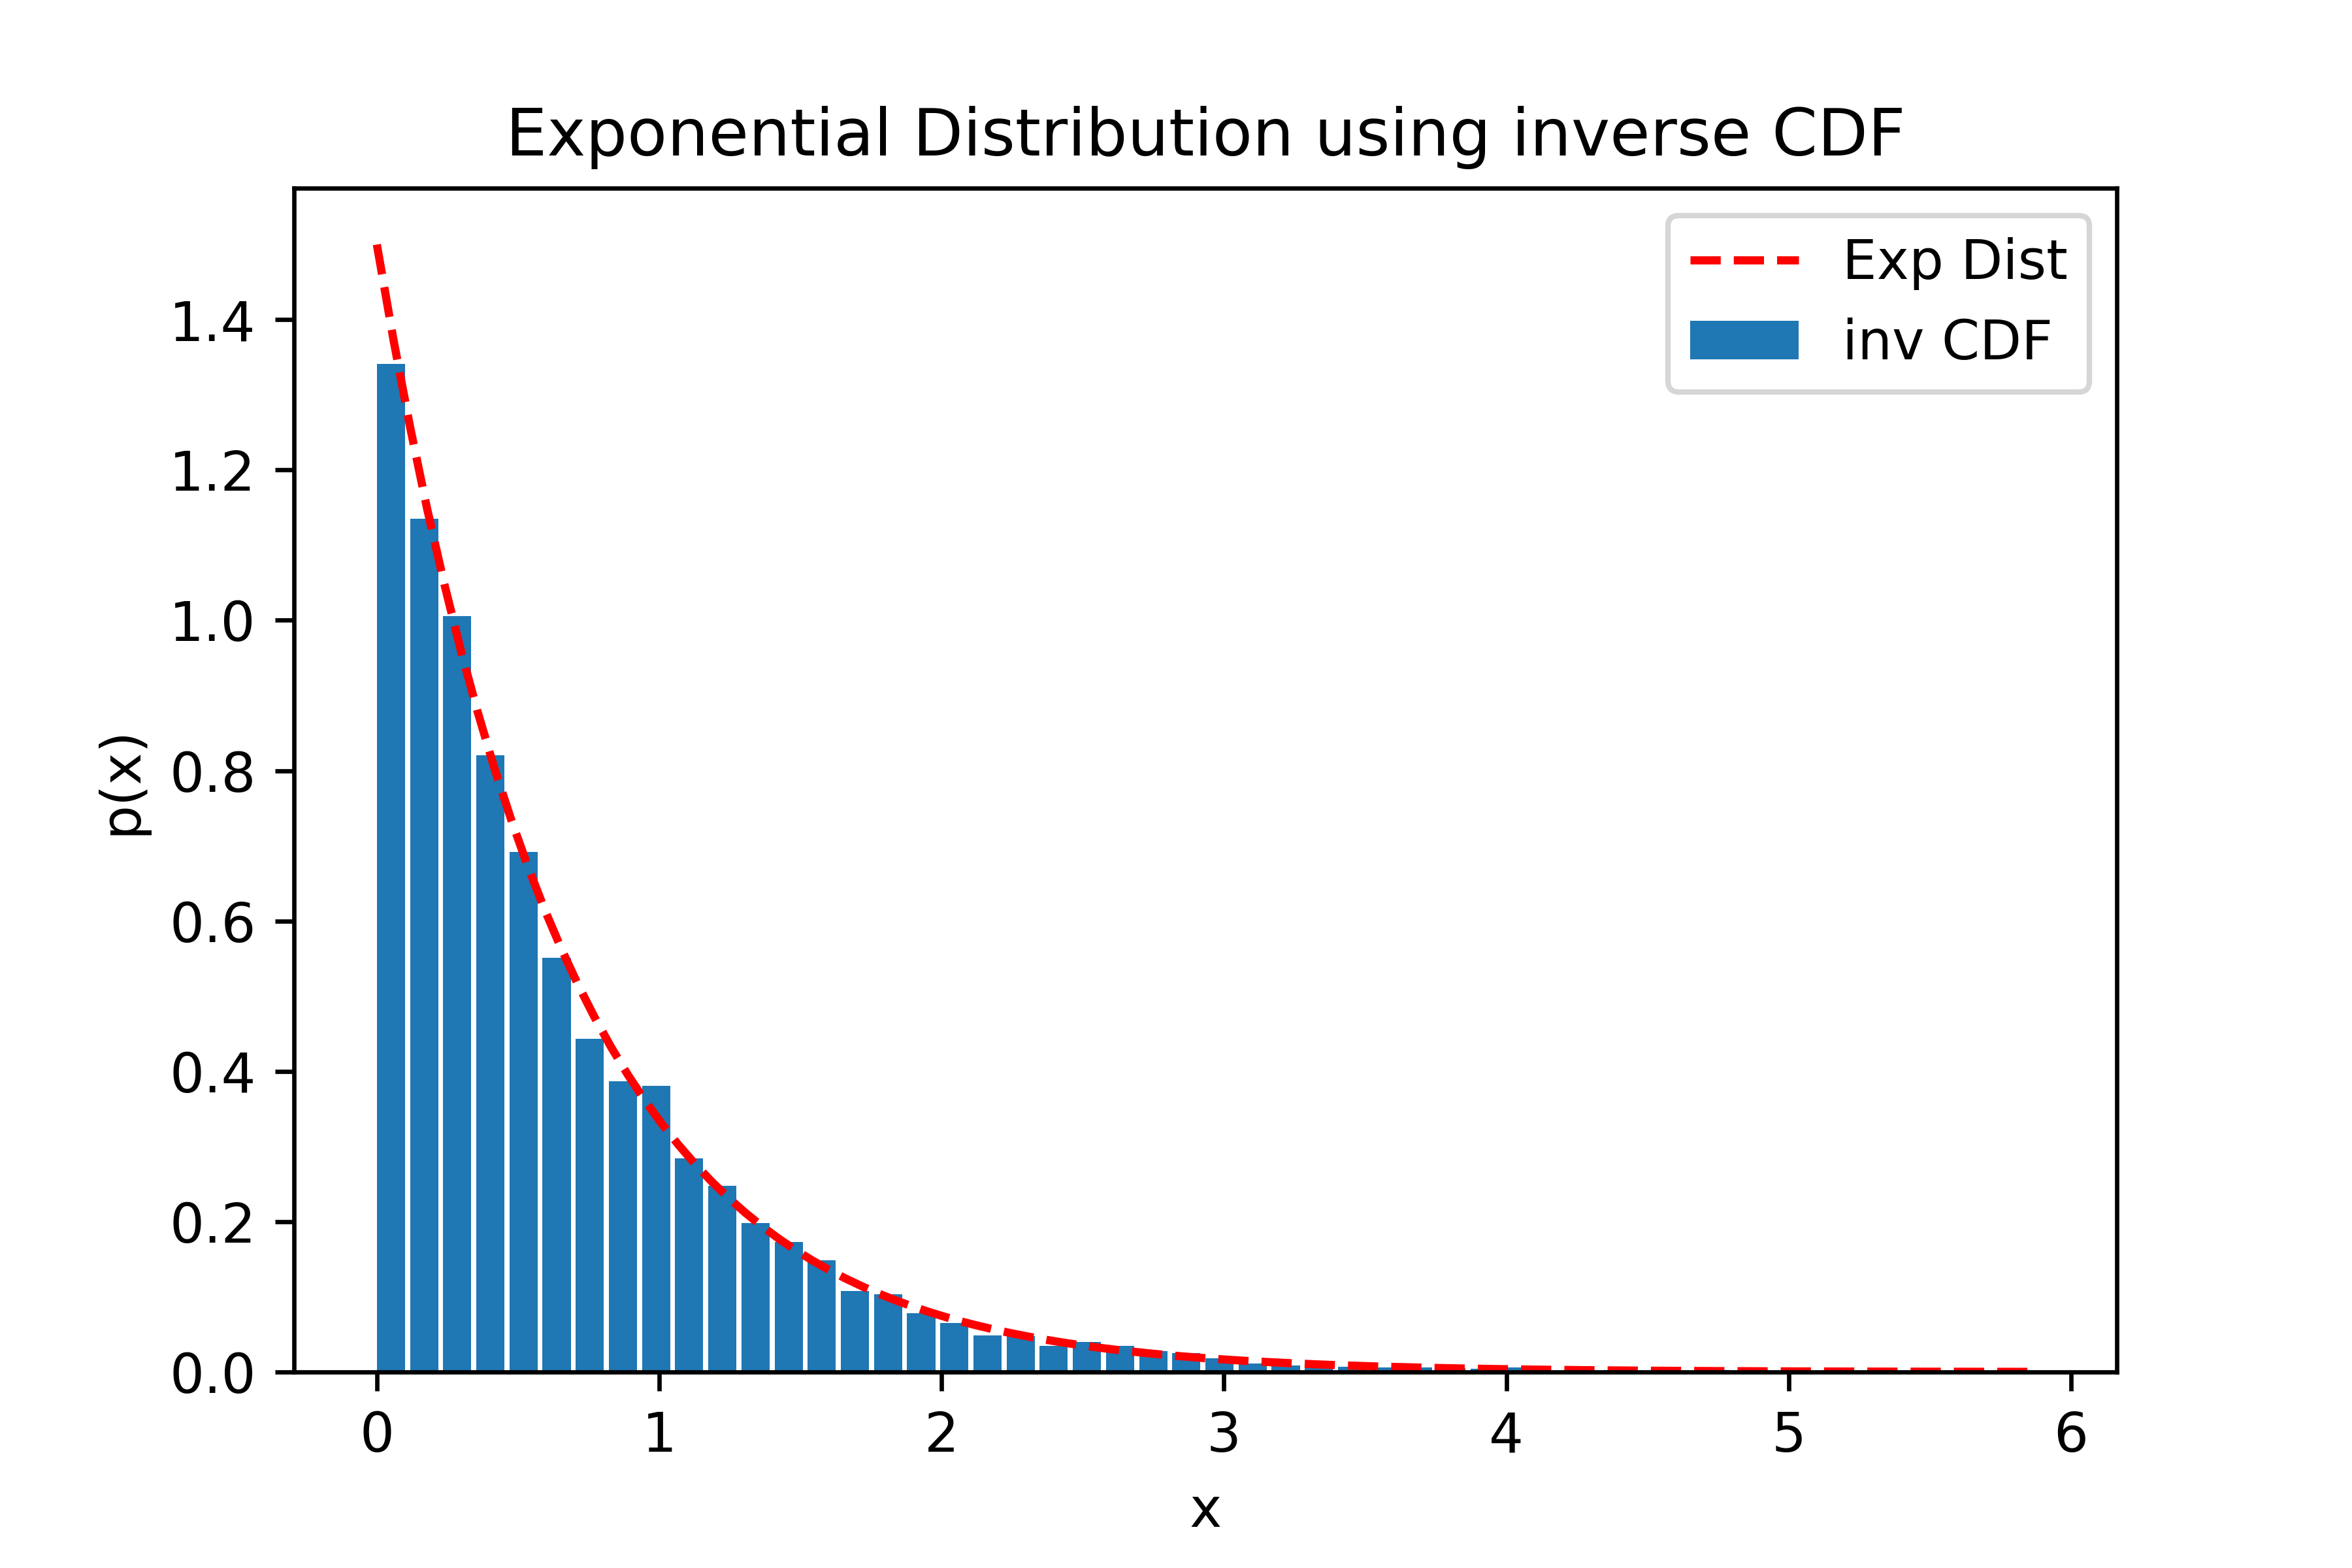
\includegraphics[width=.95\linewidth]{plot_p6_exp.png}
            \caption{$E(x; \lambda = 1.5)$}
            \label{fig:p6-cdfinv-pdf-exp}
        \end{subfigure}
        \begin{subfigure}{.45\linewidth}
            \centering
            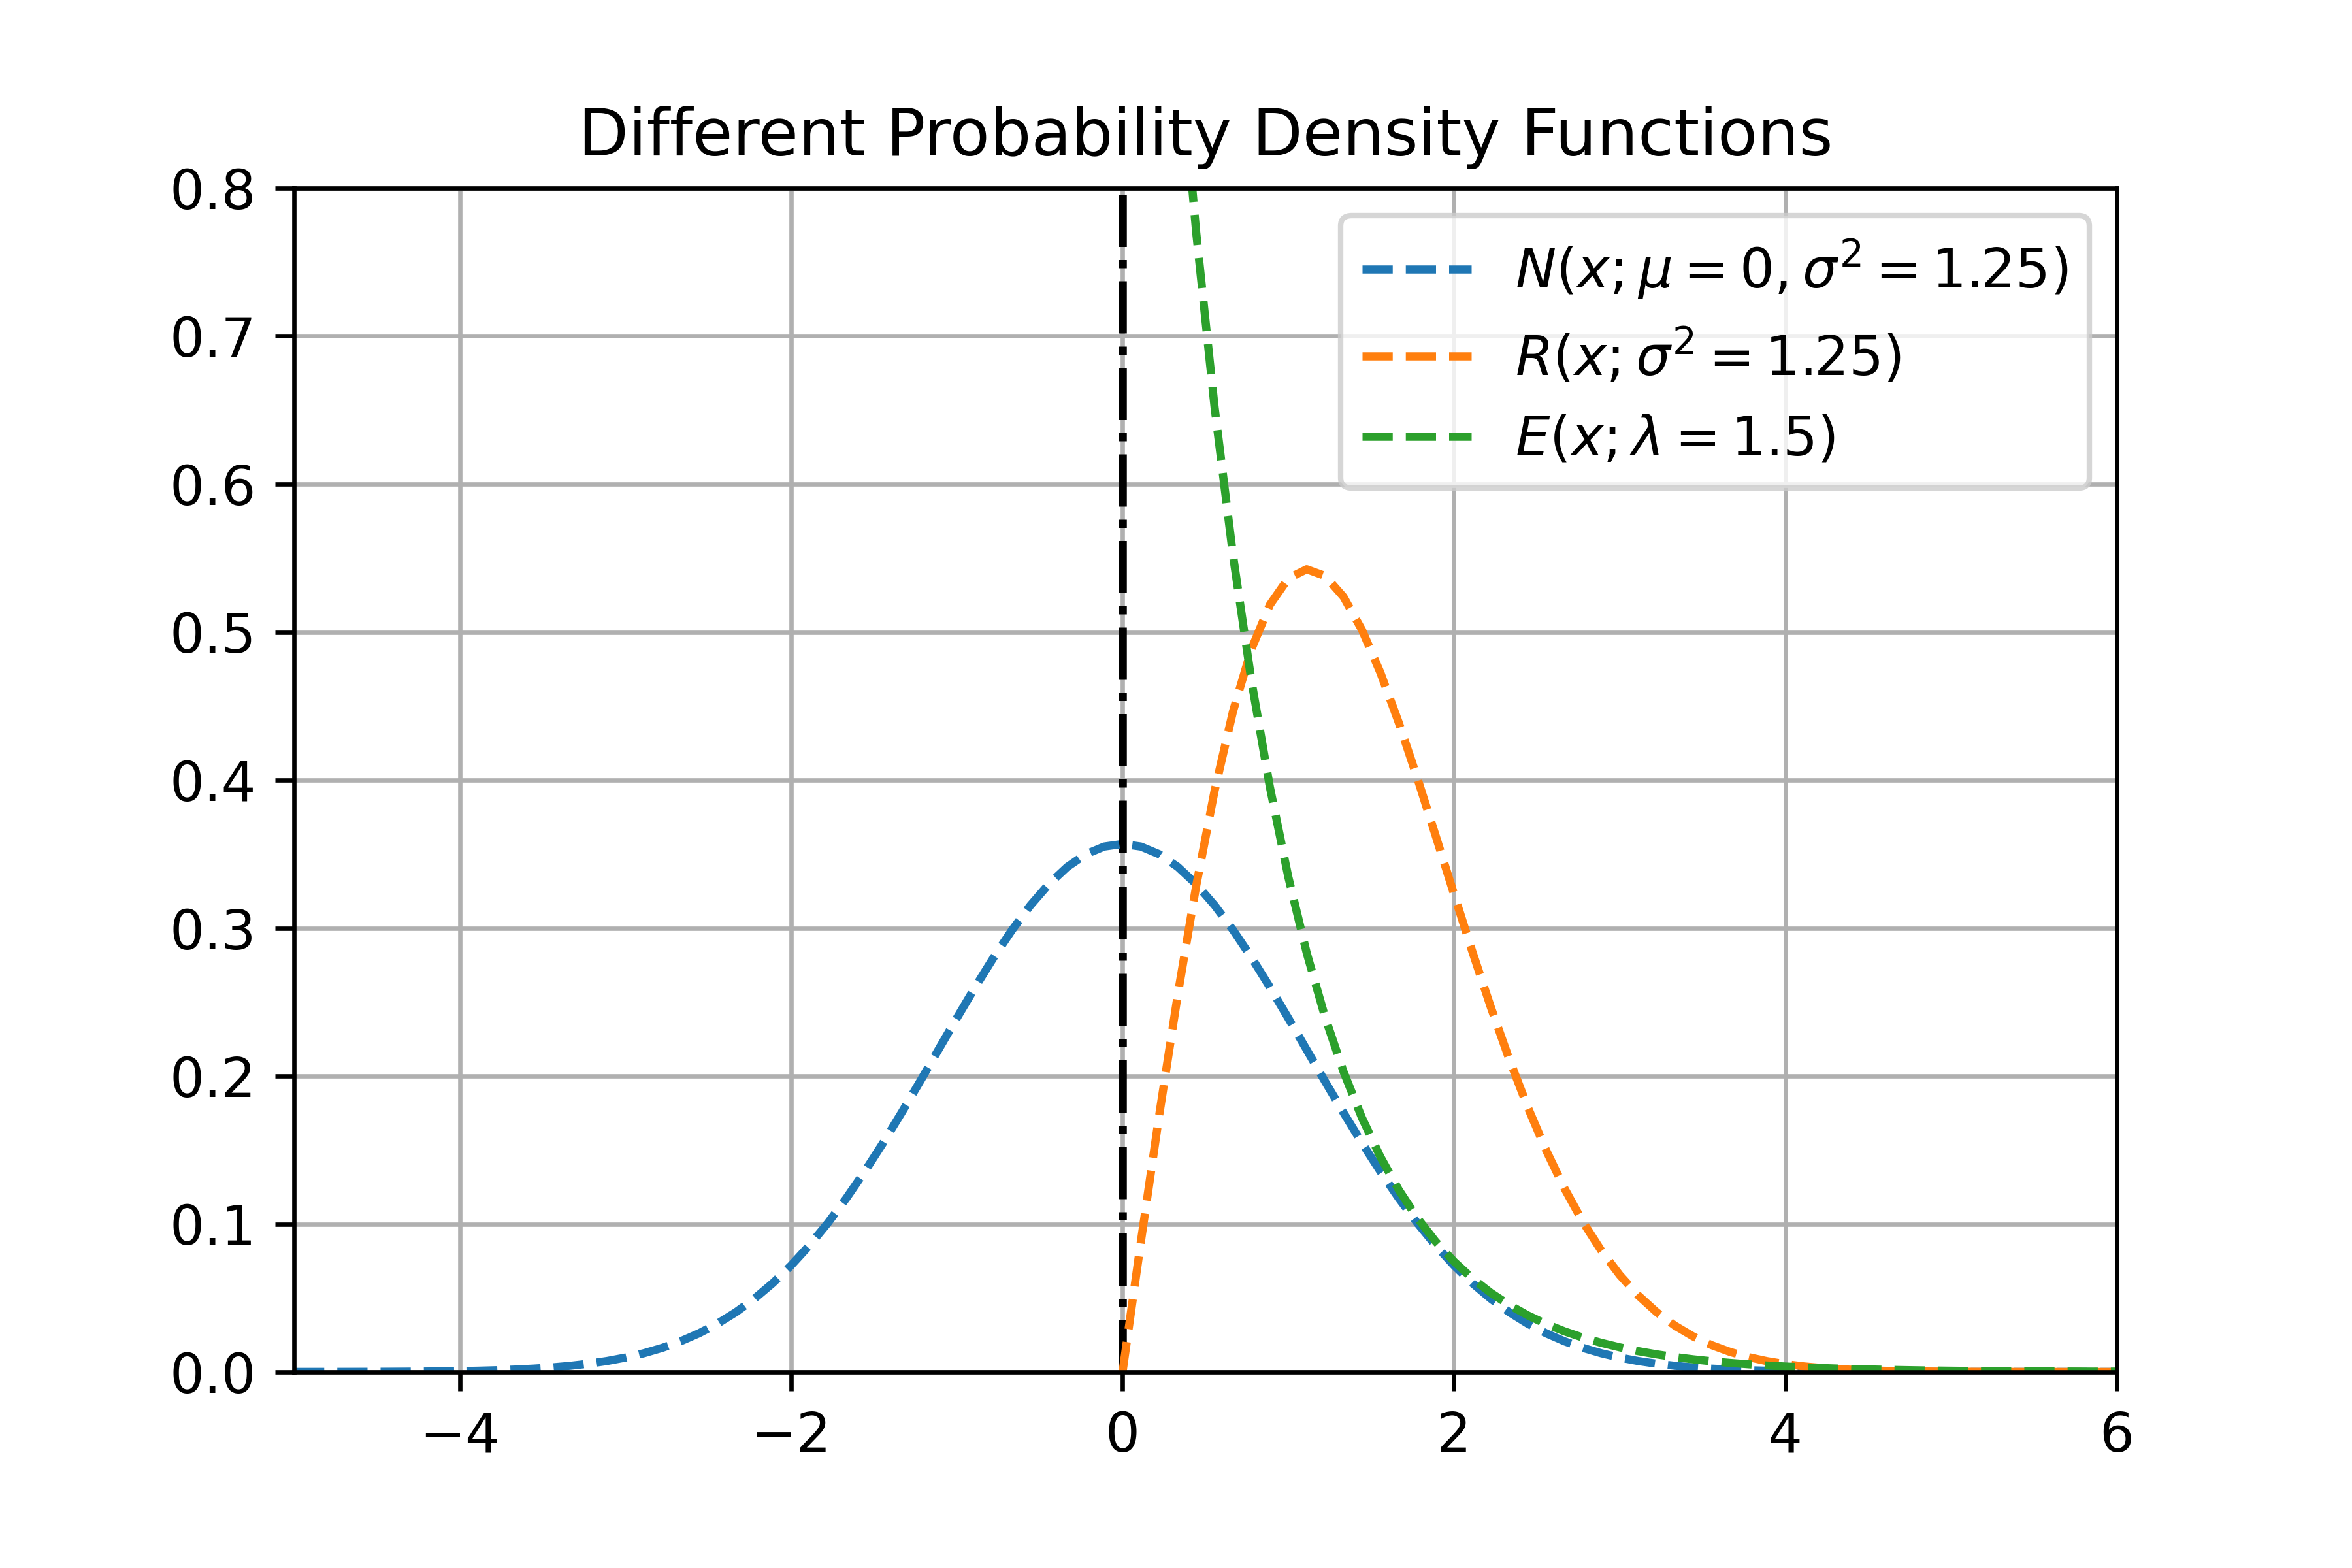
\includegraphics[width=.95\linewidth]{plot_p6_all.png}
            \caption{$N$, $R$ and $E$ PDFs}
            \label{fig:p6-subfig-all-pdfs}
        \end{subfigure}
        \caption[Visualizing PDFs as inverse of CDFs]{Using the inverse of CDFs to generate a PDF}
        \small
        Figure \ref{fig:p6-cdfinv-pdf-normal} consists of the \emph{normal distribution} generated through inverse CDF in 50 bins (as blue bars) and the actual normal PDF through function (as red dotted line). Code for this is in \ref{app:code-p6-normal}.
        Figure \ref{fig:p6-cdfinv-pdf-rayleigh} consists of the \emph{rayleigh distribution} generated through inverse of CDF (as blue bars) and the actual rayleigh PDF through function (as red dotted line). Code for this is in \ref{app:code-p6-rayleigh}.
        Figure \ref{fig:p6-cdfinv-pdf-exp} consists of the \emph{exponential distribution} generated through inverse of CDF (as blue bars) and the actual exponential PDF through function (as red dotted line). Code for this is in \ref{app:code-p6-exp}.
        Figure \ref{fig:p6-subfig-all-pdfs} consists of all three PDFs (with different parameters) in one plot, just for comparison. The \emph{Normal PDF} shown in blue line has $\mu=0$ and $\sigma^2=1.25$, the \emph{Rayleigh PDF} shown in orange line has $\sigma^2=1.25$, and the \emph{Exponential PDF} shown in green line has $\lambda=1.5$. The code responsible for this is mentioned in Appendix \ref{app:code-p6-all}
        \label{fig:p6-cdfinv-pdf}
    \end{figure}
\end{document}